\documentclass[10pt,twocolumn,letterpaper]{article}

\usepackage{cvpr}
\usepackage{microtype}
\usepackage{times}
\usepackage{epsfig}
\usepackage{graphicx}
\usepackage{amsmath}
\usepackage{amssymb}
\usepackage{caption}
\usepackage{subcaption}
\usepackage{booktabs}
\usepackage{floatrow}
\newfloatcommand{capbtabbox}{table}[][\FBwidth]
% Include other packages here, before hyperref.

% If you comment hyperref and then uncomment it, you should delete
% egpaper.aux before re-running latex.  (Or just hit 'q' on the first latex
% run, let it finish, and you should be clear).
\usepackage[pagebackref=true,breaklinks=true,letterpaper=true,colorlinks,linkcolor=blue,citecolor=blue,bookmarks=false]{hyperref}

\newcommand{\JT}[1]{\textcolor{blue}{JT: #1}}
\newcommand{\HP}[1]{\textcolor{red}{HP: #1}}
\newcommand{\DFH}[1]{\textcolor{red}{DH: #1}}

% \cvprfinalcopy % *** Uncomment this line for the final submission

\def\cvprPaperID{0947} % *** Enter the CVPR Paper ID here
\def\httilde{\mbox{\tt\raisebox{-.5ex}{\symbol{126}}}}

% Pages are numbered in submission mode, and unnumbered in camera-ready
\ifcvprfinal\pagestyle{empty}\fi
\begin{document}

%%%%%%%%% TITLE
\title{Guided Proofreading of Automatic Segmentations for Connectomics\\~\\\textit{Supplemental Material}}

\author{Daniel Haehn\\
Institution1\\
Institution1 address\\
{\tt\small haehn@seas.harvard.edu}
% For a paper whose authors are all at the same institution,
% omit the following lines up until the closing ``}''.
% Additional authors and addresses can be added with ``\and'',
% just like the second author.
% To save space, use either the email address or home page, not both
\and
Second Author\\
Institution2\\
First line of institution2 address\\
{\tt\small secondauthor@i2.org}
}

\maketitle
%\thispagestyle{empty}

%%%%%%%%% ABSTRACT

%%%%%%%%% BODY TEXT

\section{Classifier}

\subsection{CNN Architecture}
2 vs 4 layers vs resnet

\subsection{Training Parameters}

\subsection{Automatic Method Threshold $p_t$}

\section{L. Cylinder Results}

\begin{figure}[t]
\centering
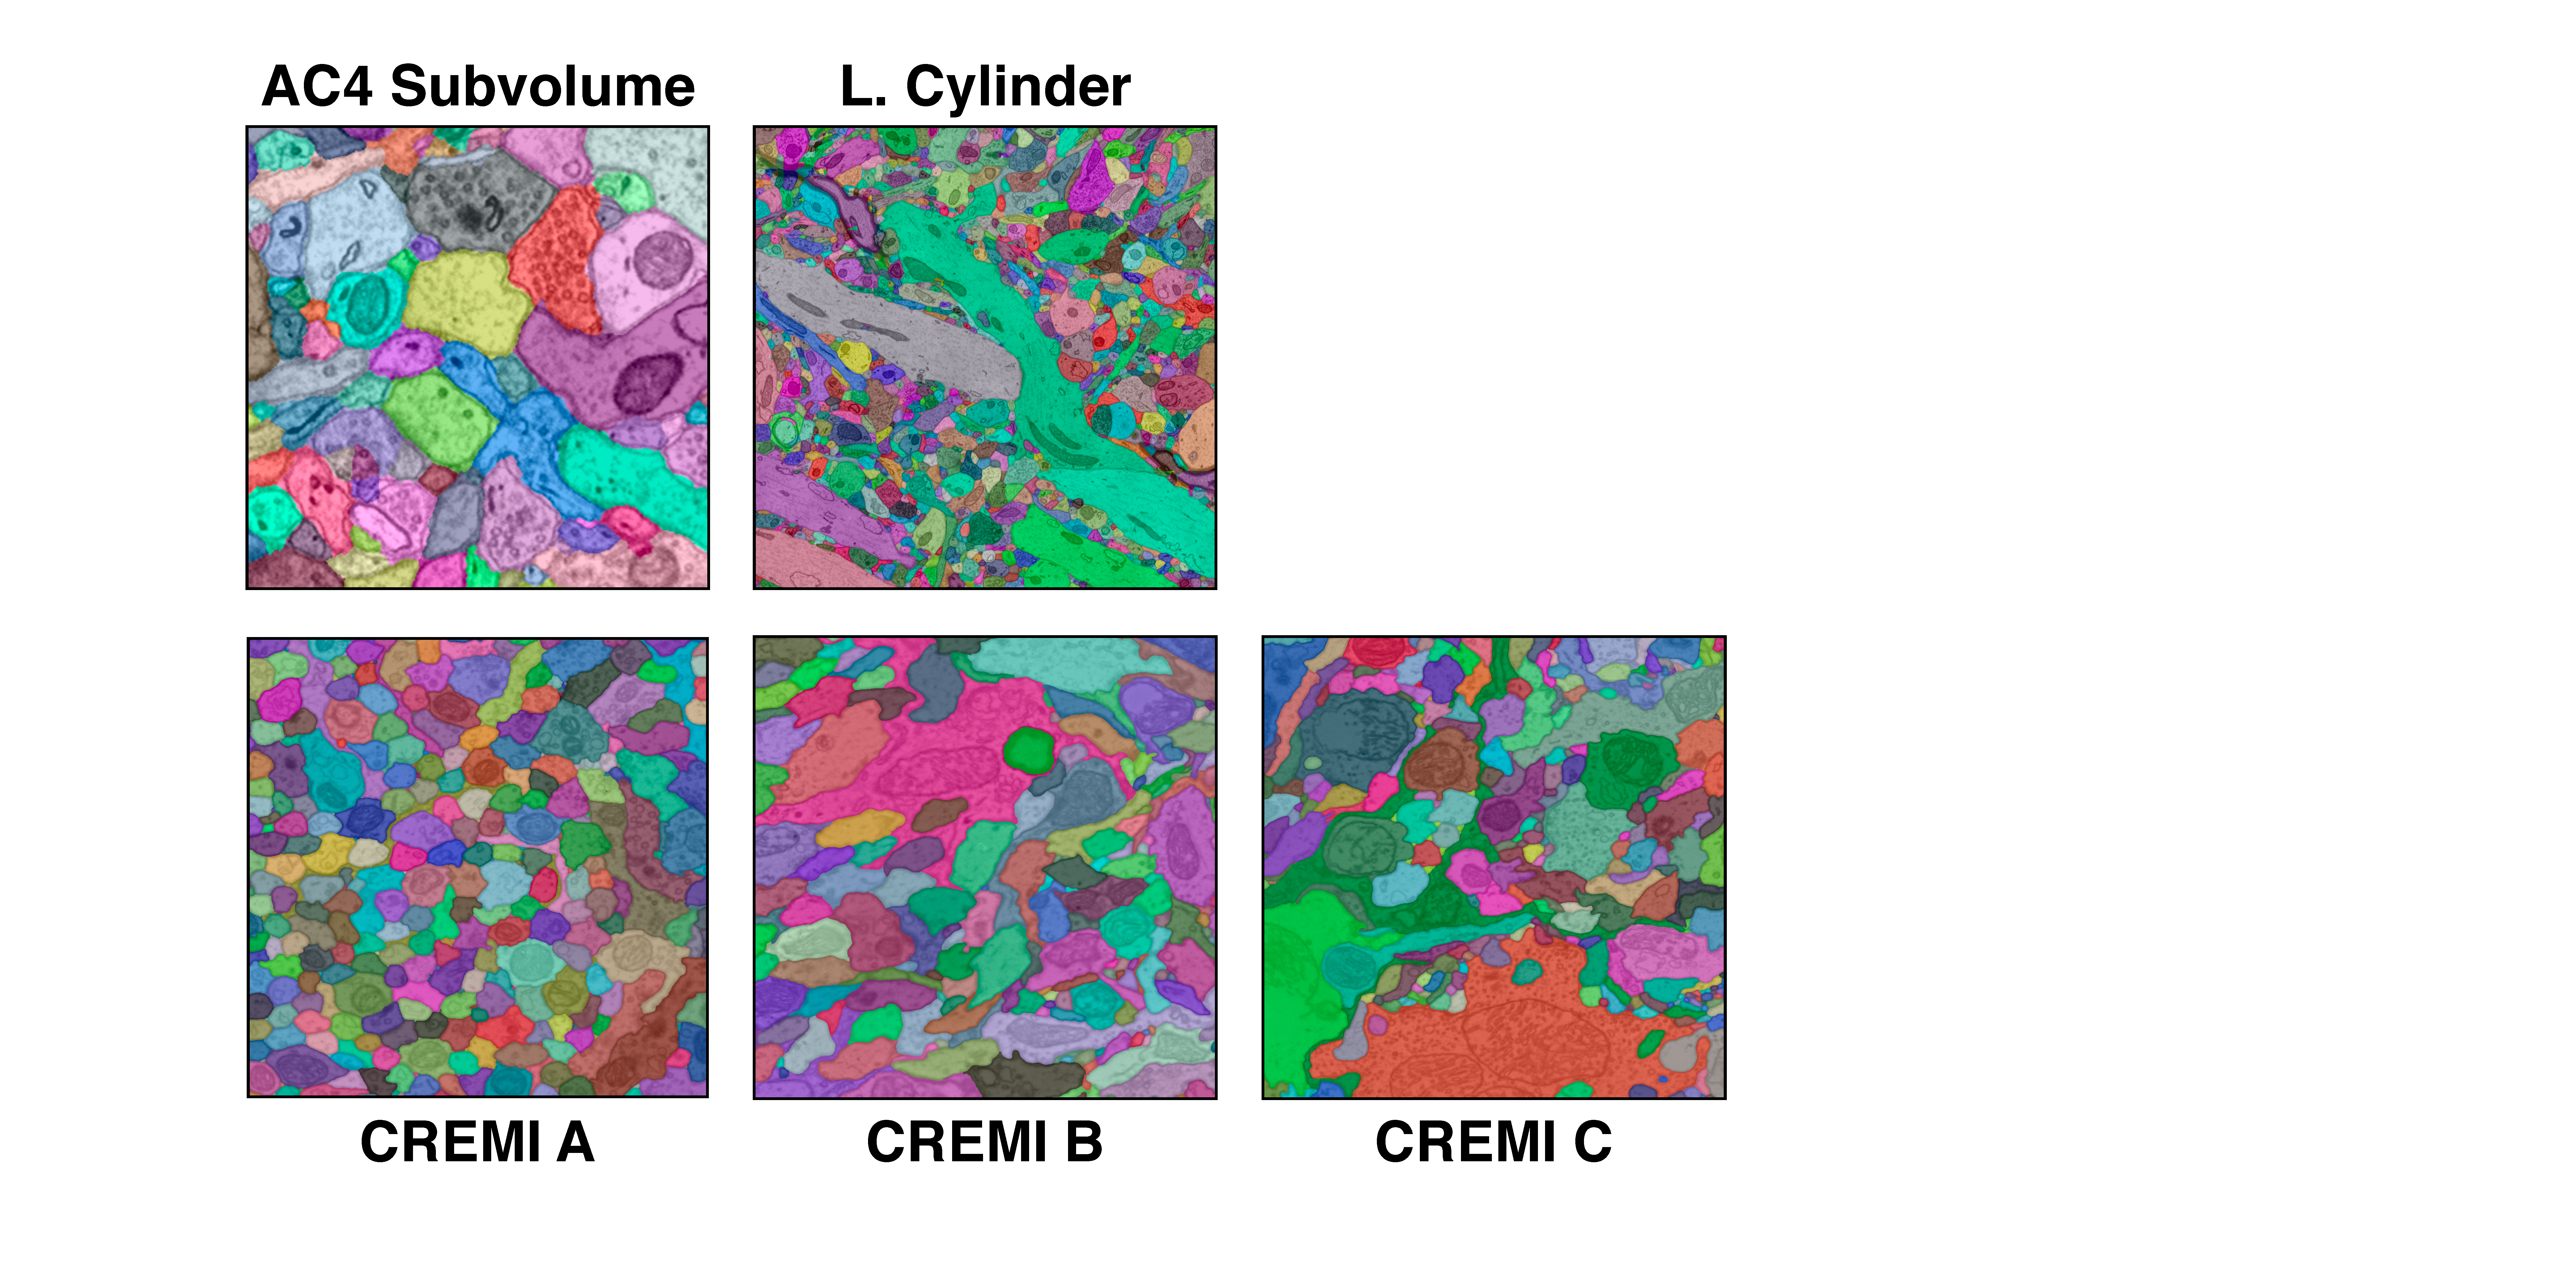
\includegraphics[width=\linewidth]{gfx/datasets.png}
\caption{The five different datasets we use for evaluation. The top row shows the first slice of the AC4 and L.~Cylinder mouse brain datasets as reported in the paper. The bottom row shows the first slice of the CREMI A/B/C fruit fly datasets which we used for additional experiments.}
\label{fig:datasets}
\end{figure}

We report experiments and results on the L.~Cylinder dataset in the paper. Figure~\ref{fig:cyltrails} and~\ref{fig:cylboxplot} visualize the reported results measured as variation of information (VI). We compare automatic selection with threshold and selection oracle using focused proofreading and guided proofreading.

\paragraph{Best possible VI.} The selection oracle using guided proofreading does not reach the best possible VI score. We calculate this score by intersecting the initial segmentation and the ground truth. In theory, the classifier should be able to reach this lower bound. However, due to the classification patch size, the membrane probability maps we used included a 30 pixel frame region. Guided proofreading ignores all segments within this frame region, and so cannot reach the best possible VI in some datasets.

\begin{figure}[t]
\centering
\includegraphics[width=\linewidth]{gfx/cyl_trails.pdf}
\caption{Performance comparison of Plaza's focused proofreading and our guided proofreading on the L.~Cylinder dataset as reported in the paper. All measurements are shown as median VI, the lower the better. We compare automatic selection with threshold ($p_t=0.95$, green line) and the selection oracle for accepting or rejecting corrections using each method. Guided proofreading yields better results faster with fewer corrections.}
\label{fig:cyltrails}
\end{figure}

\begin{figure}[t]
\centering
\includegraphics[width=\linewidth]{gfx/cylboxplot.pdf}
\caption{VI distributions of guided proofreading (GP) and focused proofreading (FP) output across slices of the L.~Cylinder dataset, with different error correction approaches. The variation resulting from performance of FP with automatic selection is $7.8\times$ higher than GP (\protect\includegraphics[width=0.2cm]{gfx/arrow.pdf}), with median VI of $2.75$ and $SD=0.789$.}
\label{fig:cylboxplot}
\end{figure}

\section{Confirmatory Data Analysis} 

We use a single factor between-subject design with the factor being the proofreading method (GP, FP, or Dojo). Our hypothesis is that VI reduction is significantly better with GP than with other tools. For this, we treat VI as a continuous variable and use analysis of variance (ANOVA~\cite{shaffer1995}) followed by parametric tests (Welch's t-test~\cite{welch}).

\paragraph{AC4 subvolume.} For novice performance, we observe a significant effect ($\alpha=0.05$) of which proofreading tool is used for the three conditions GP, FP, and Dojo [$F(2,27) = 6.446, p = 0.005$] when comparing the mean VI outcome. Post hoc comparisons (after Bonferroni correction) indicate that the mean VI for GP is significantly lower than for FP [$t_{27} = -2.7696, p = 0.0168$], and that the mean VI for GP is significantly lower than for Dojo [$t_{27} = -4.407, p < 0.001$]. This means that novices using GP perform significantly better than using FP and Dojo.
A similar trend is visible when comparing the expert performance between GP and FP as the change in mean VI of GP is significantly better ([$F(1,18) = 7.054, p = 0.016$] and [$t_{18} = -2.6559, p = 0.0216$]). For automatic selection with threshold, the difference in mean VI is very large and GP also performs significantly better ([$F(1,18) = 89.902, p < 0.001$] and [$t_{18} = 9.482, p < 0.001$]). The final VI scores of the selection oracle with GP and FP are very similar and the difference between them is not significant [$F(1,18) = 0.795, p = 0.384$]. However, the VI reduction rate of GP is much higher (Fig.~6, main paper, right).

\vspace{-4mm}

\paragraph{L. Cylinder.} The automatic selection with threshold yields similar results as on the AC4 dataset, and we observe a significant improvement when using GP instead of FP ([$F(1,98) = 26.676, p < 0.001$], post hoc comparison [$t_{98} = 5.1648, p < 0.001$]). The selection oracles of GP and FP result in very similar final VI scores and the difference is not significant [$F(1,98) = 0.071, p = 0.790$], but GP reaches minimum VI faster in $10,000$ corrections versus FP in $26,170$ corrections.
    
    
\section{Additional Experiments}
\label{sec:addexp}

\paragraph{CREMI A/B/C.} As part of the MICCAI 2016 challenge on circuit reconstruction from electron microscopy images (CREMI), six ssTEM datasets were made publicly available\footnote{\scriptsize{\url{http://www.cremi.org}}},  each $1250\times1250\times125$ voxels. Since only three datasets include manually-labeled `ground truth', we use these three volumes for our experiments. The volumes are part of an adult fruit fly (Drosophila melanogaster) brain. The resolution of all three datasets is $4\times4\times40~\text{nm}^3\text{/voxel}$. We evaluate error detection and correction on subvolumes of CREMI A/B/C with the dimensions $1250\times1250\times5$ voxels. The subvolumes were cut from the last 25 sections of each of the three datasets and unseen during training. We compare focused proofreading and guided proofreading with automatic selection ($p_t=0.95$) and selection oracle.

\paragraph{Retraining.} Since the CREMI data is a different species, we simply retrain our split error classifier as well as focused proofreading by Plaza~\cite{focused_proofreading}. For this, we use the first 100 sections of each of the three CREMI datasets combined as training data. All parameters are unchanged and left as reported in the paper. 

\begin{figure}[t]
\centering
\includegraphics[width=\linewidth]{gfx/cremi_roc_separate_small.pdf}
\caption{Receiver Operating Characteristic curves comparing focused proofreading and guided proofreading automatic correction on the CREMI A/B/C fruit fly subvolumes. Guided proofreading performs better on all three datasets.}
\label{fig:cremi_performance}
\end{figure}

\paragraph{Classification Performance.} Figure~\ref{fig:cremi_performance} compares the  focused proofreading and guided proofreading classifiers on the CREMI A/B/C datasets. Our method exhibits higher sensitivity and lower fall-out.

%\paragraph{Error correction.} In all three datasets merge error detection found over 300 merge errors. Unfortunately, merge error correction crashed because of a software error on our part. Therefore, we only evaluate split error detection and correction on subvolumes of CREMI A/B/C with the dimensions $1250\times1250\times5$ voxels. The subvolumes were cut from the last 25 sections of each of the three datasets and unseen during training. We compare focused proofreading and guided proofreading with automatic selection ($p_t=0.95$) and selection oracle.

\subsection{CREMI A}

\begin{figure}[t]
\centering
\includegraphics[width=\linewidth]{gfx/cremiA_trails.pdf}
\caption{Performance comparison of Plaza's focused proofreading and our guided proofreading on 5 sections of the CREMI A dataset. All measurements are reported as median VI, the lower the better. The threshold for automatic selection is $p_t=0.95$ (green line). The slope of the selection oracle shows that guided proofreading reduces VI faster.}
\label{fig:cremiAtrails}
\end{figure}

\begin{figure}[t]
\centering
\includegraphics[width=\linewidth]{gfx/cremiAboxplot.pdf}
\caption{VI distributions of guided proofreading (GP) and focused proofreading (FP) output across slices of the CREMI A dataset, with different error correction approaches. The variation resulting from performance of FP with automatic selection is $5.4\times$ higher than GP (\protect\includegraphics[width=0.2cm]{gfx/arrow.pdf}), with median VI of $5.32$ and $SD=0.009$. GP does not reach the best possible VI as discussed in the text.}
\label{fig:cremiAboxplot}
\end{figure}

Figure~\ref{fig:cremiAtrails} and~\ref{fig:cremiAboxplot} compare Plaza's focused proofreading and guided proofreading on the five sections of CREMI A.

\vspace{-4mm}

\paragraph{Selection oracle.} With focused proofreading, the selection oracle reduces median VI to 0.928, $SD=0.043$ from an initial median VI of 1.06 ($SD=0.055$). 532 corrections out of 3707 were accepted. Guided proofreading does not reach the best possible VI, however, reduces VI faster with less corrections to 0.941 ($SD=0.04$). Out of 4463 corrections, 1275 were accepted.

\paragraph{Automatic selection with threshold.} Not surprisingly, focused proofreading performs poorly when ran automatically (VI of 5.32, $SD=0.009$). Guided proofreading is able to reduce VI to 0.989 ($SD=0.043$) with $p_t=0.95$.

\subsection{CREMI B}

Figure~\ref{fig:cremiBtrails} and~\ref{fig:cremiBboxplot} show the results on the CREMI B dataset.

\paragraph{Selection oracle.} Focused proofreading is able to reduce median VI to 1.29, $SD=0.031$ from an initial median VI of 1.63 ($SD=0.025$). Out of 1959 corrections, the selection oracle accepted 517. With guided proofreading, the median VI is reduced to 1.30, $SD=0.03$ while accepting 1111 corrections out of 3073.

\paragraph{Automatic selection with threshold.} Focused proofreading results in a VI of 4.25 ($SD=0.07$). Guided proofreading reduces median VI to 1.43 ($SD=0.038$).

\begin{figure}[t]
\centering
\includegraphics[width=\linewidth]{gfx/cremiB_trails.pdf}
\caption{Split error correction by Plaza's focused proofreading and our guided proofreading compared on the CREMI B dataset. All measurements are reported as median VI, the lower the better. Automatic selection with threshold (green line) yields reasonable performance using guided proofreading.}
\label{fig:cremiBtrails}
\end{figure}

\begin{figure}[t]
\centering
\includegraphics[width=.9\linewidth]{gfx/cremiBboxplot.pdf}
\caption{VI distributions of guided proofreading (GP) and focused proofreading (FP) output across 5 sections of the CREMI B dataset. We compare automatic selection and oracle selection. The variation resulting from performance of FP with automatic selection is $3\times$ higher than GP (\protect\includegraphics[width=0.2cm]{gfx/arrow.pdf}), with median VI of $4.25$ and $SD=0.07$.}
\label{fig:cremiBboxplot}
\end{figure}

\subsection{CREMI C}

The results of split error correction using focused proofreading and guided proofreading on the CREMI C subvolume are shown in Figure~\ref{fig:cremiCtrails} and~\ref{fig:cremiCboxplot}.

\paragraph{Selection oracle.} With focused proofreading, the initial median VI of 1.75 ($SD=0.086$) is reduced to 1.45 ($SD=0.056$) with 670 accepted corrections out of 2694. Guided proofreading is able to reduce the VI to 1.47 ($SD=0.06$). Here, the oracle accepted 1531 out of 4332 corrections. 

\paragraph{Automatic selection with threshold.} Focused proofreading results in a VI of 4.81 ($SD=0.03$). Guided proofreading with $p_t=0.95$ reduces median VI to 1.57 ($SD=0.081$).

\begin{figure}[t]
\centering
\includegraphics[width=\linewidth]{gfx/cremiC_trails.pdf}
\caption{Performance comparison of Plaza's focused proofreading and our guided proofreading on the CREMI C dataset. Lower VI scores are better. Guided proofreading corrects the initial segmentation faster with less corrections than focused proofreading. The green line shows the automatic threshold $p_t=0.95$.}
\label{fig:cremiCtrails}
\end{figure}

\begin{figure}[t]
\centering
\includegraphics[width=\linewidth]{gfx/cremiCboxplot.pdf}
\caption{VI distributions of guided proofreading (GP) and focused proofreading (FP) output across the CREMI C subvolume, with different error correction approaches. The variation resulting from performance of FP with automatic selection is $3\times$ higher than GP (\protect\includegraphics[width=0.2cm]{gfx/arrow.pdf}), with median VI of $4.81$ and $SD=0.08$.}
\label{fig:cremiCboxplot}
\end{figure}
\section{Forced Choice User Experiment}

\subsection{Recruitment and Participation}

flyers, participant list

\subsection{Example Classifications}

Where did users make a mistake?

\subsection{Subjective Responses}

NASA TLX ANOVA analysis

%\newpage~\newpage
{\small
\bibliographystyle{ieee}
\bibliography{connectomics}
}

\end{document}
